\begin{blocksection}
\question Fill in each blank in the code example below so that its environment diagram is the following. You do not need to use all the blanks.

\begin{multicols}{2}
\begin{lstlisting}
fruit = [1, 2, [3, 4]]
fruit._______________________
fruit[3][2]._________________
fruit[2][2]._________________
fruit[3][3][2][2][2][1] = ___
\end{lstlisting}

\columnbreak
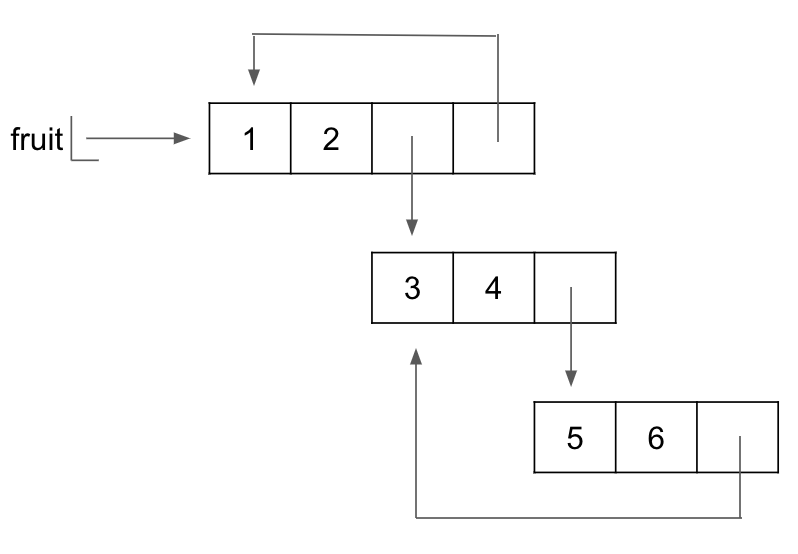
\includegraphics[width=.45\textwidth]{fruit_loops.png}
\end{multicols}

\begin{solution}[2in]
\begin{lstlisting}
fruit = [1, 2, [3, 4]]
fruit.append(fruit)
fruit[3][2].append([5, 6])
fruit[2][2].append(fruit[2])
fruit[3][3][2][2][2][1] = 4
\end{lstlisting}
\end{solution}
\end{blocksection}
